\documentclass[conference]{IEEEtran}

\usepackage[british]{babel}
\usepackage{cite}
\usepackage{graphicx}
\usepackage{tabularx}
\usepackage[hyphens]{url}
\usepackage{amsthm}
\theoremstyle{definition}
\newtheorem{definition}{Definition}
\usepackage[textstyle,squaren]{SIunits}
%\usepackage[pdftex,colorlinks=true]{hyperref}


% correct bad hyphenation here
%\hyphenation{op-tical net-works semi-conduc-tor}


\begin{document}
%
% paper title
\title{Measuring UK Crime Gangs}

% author names and affiliations
% use a multiple column layout for up to three different
% affiliations
\author{\IEEEauthorblockN{Giles Oatley}
\IEEEauthorblockA{Department of Computing\\
Cardiff Metropolitan University\\
Cardiff, UK\\
Email: goatley@cardiffmet.ac.uk}
\and
\IEEEauthorblockN{Tom Crick}
\IEEEauthorblockA{Department of Computing\\
Cardiff Metropolitan University\\
Cardiff, UK\\
Email: tcrick@cardiffmet.ac.uk}}

% conference papers do not typically use \thanks and this command
% is locked out in conference mode. If really needed, such as for
% the acknowledgment of grants, issue a \IEEEoverridecommandlockouts
% after \documentclass


% use for special paper notices
%\IEEEspecialpapernotice{(Invited Paper)}


% make the title area
\maketitle


\begin{abstract}
This paper describes the output of a study to tackle the problem of
gang-related crime in the UK; we present the intelligence and
routinely gathered data available to a UK regional police force, and
describe an initial social network analysis of gangs in the Greater
Manchester area of the UK between 2000-2006. By applying social
network analysis techniques, we attempt to detect the birth of two new
gangs based on local features (modularity, cliques) and global
features (clustering coefficient). Thus for the future, identifying
the changes in these can help us identify the possible birth of new
gangs (sub-networks) in the social system. Furthermore, we study the
dynamics of these networks globally and locally, and have identified
the global characteristics that tell us that they are not random
graphs -- they are small world graphs -- implying that the formation
of gangs is not a random event. However, we are not yet able to
conclude anything significant about scale-free characteristics due to
insufficient sample size.
\end{abstract}

% For peer review papers, you can put extra information on the cover
% page as needed:
% \ifCLASSOPTIONpeerreview
% \begin{center} \bfseries EDICS Category: 3-BBND \end{center}
% \fi
%
% For peerreview papers, this IEEEtran command inserts a page break and
% creates the second title. It will be ignored for other modes.
\IEEEpeerreviewmaketitle


\section{Introduction}\label{sec:introduction}

We present the dynamics of a social network study of gang activity in
Greater Manchester, a region in the north of the UK. We use the
intelligence gathered by police observations of known gang members and
associated criminals. We develop the statistical analysis of network
dynamics, combining well-known global topological measures, local
motifs and
modules~\cite{CostaRodriguesTraviesoVillasBoas2007,Jackson2008,Newman2003}.
Network motifs are subgraphs that appear more frequently in a real
network than could be statistically expected. At a global level, if
these networks of associations exhibit clustering behaviour this
indicates the presence of gangs. At a local level, any defined
substructures will provide us information about the gang structure. We
are interested in modelling the dynamics of the gangs, their
development and fragmentation into new gangs, and we hope that the
study of the dynamics in such modules will provide information on the
structural changes within gangs that lead to birth of new gangs, and
predictors of other gang-related behaviour.

Furthermore, we investigate if the networks have scale-free,
small-world or other characteristics
\cite{Watts1999,AlbertBarabasi2002,Newman2003}; small-world networks
are characterised by a diameter that grows logarithmically with their
size. One important characteristic of the small-world phenomenon is
that each pair of nodes are connected through a relatively small
number of steps to a huge network size defined by the total number of
nodes. Scale-free structures consists of many nodes with low degrees
and a few hubs with high
degrees~\cite{AlbAlbNak04,CostaRodriguesTraviesoVillasBoas2007,Jackson2008}. If
the offender networks can be classified into either (or both) of these
categories (or other known network types), then this provides not only
insight into the dynamics of the gang network, but also operational
uses; for instance, network disruption/destruction strategies,
nodes/offenders to monitor, and so on.


\section{Problem description and data}\label{sec:problemdescription}


Numerous shootings -- both fatal and non-fatal -- have taken place
over the years as the the Pepperhill, Gooch, Doddington and Longsight
Crew gangs (see Table~\ref{table:gangnames}) have clashed over drug
territories and other disputes. Many of these gun fire exchanges were
on public streets, some were planned acts and some were spontaneous
events.

\begin{table}[htb]
\centering
\begin{tabularx}{\columnwidth}{c X c}
%\begin{tabular}{c c c} 
\hline
Gang label & Gang Name & Formation  \\ %[0.5ex]
\hline
A & Gooch & 1990s\\
B & Doddington/Pepperhill & 1990s\\
C & Longsight Crew &  c.2001\\
D & Rusholme Crew Gangsters & c.2004\\ %[1ex] % [1ex] adds vertical space 
\hline
%\end{tabular}
\end{tabularx}
\caption{Gang names and approximate dates of formation.}
\label{table:gangnames}
\end{table}

In 2001, a new approach to tackling gun crime began to develop with
police working more closely with the local community and other
agencies. The Manchester Multi-Agency Gang Strategy (MMAGS), a
multi-agency approach to tackling gun crime and detering young people
from entering into a gang/gun culture was initiated as a result of a
UK Home Office report~\cite{BullockTilley2002}. The report concludes
that about 60 per cent of shootings are thought to gang-related, with
violence in general, and gun violence and fatal shootings inparticular
are concentrated in specific small areas of South Manchester, and that
gangs in South Manchester are loosely turf-based.

The geographical proximity between Gangs A and B is hundreds of meters, literally a few streets
away from each other.  Gangs A and B show a negative attitude towards
each other, often resulting in `tit-for-tat' gun crimes. The alignment
between Gangs A and D is possibly because of a mutual rivalry with B,
while the positive alignment of B with C is because A has encroached
on C's `territory' for drug sales. Agreeing strongly with the Home Office
report~\cite{BullockTilley2002} we find: 38\% (n=162) of all serious
crimes occurring within \unit{1}{\kilo\meter} radius (of gang
locations) and 63\% of all serious crimes occur within
\unit{2}{\kilo\meter}, and 53\% (n=9) of murders are within
\unit{3}{\kilo\meter}; 38\% (n=34) of attempted murders are within
\unit{1}{\kilo\meter} and 63\% within \unit{2}{\kilo\meter}; and, 33\%
(n=17) of serious woundings are within \unit{1}{\kilo\meter} and 48\%
are within \unit{2}{\kilo\meter}.



\section{Police databases}\label{sec:policedatabases}

The database used for this analysis included the list of associates
for each gang member, with fields such as unique identifiers for each
offender, date of birth, relationship between the offenders, ethnic
origin, reason reported and date of occurrence.

%\subsection{Link types}\label{sec:linktypes}
The network links available are quite different to other existing work
with networks of burglars or retail fraudsters
\cite{OatleyZeleznikowLearyEwart2005,OatleyMcGarryEwart2006}). These link
types are: \emph{Accomplice}; \emph{Brother-Brother};
\emph{Boyfriend}; \emph{Brother}; \emph{Sister}; \emph{Charged with};
\emph{Child}; \emph{Cohabitant}; \emph{Foster child}; \emph{Foster
parent}; \emph{Friend}; \emph{Girlfriend}; \emph{Guardian};
\emph{Other}; \emph{Parent}; \emph{Relative}; \emph{Spouse};
\emph{Sister-Sister}; \emph{Ward}; \emph{Gay Boyfriend}; and \emph{Gay
Girlfriend}.



\section{Identifying community structure}\label{sec:communitystructure}
In order to investigate community structure we removed any nodes with
less than six connections (i.e. degree 6);
Figure~\ref{fig:2002core_labelled} shows data from 2002, with the
well-established Gangs A and B, and also the newly formed Gang C (in
2001). The Gangs A, B, and C are highly interconnected, with
Figure~\ref{fig:2002core_labelled} also showing the `go-betweens',
labelled as \emph{ab*} and \emph{bc*}. Individuals who are only
connected to one gang, and who are highly connected within themselves,
are labelled \emph{a*} and \emph{b*}. In this way it is easier to see
the communities.


\begin{figure}[htb]
\centering
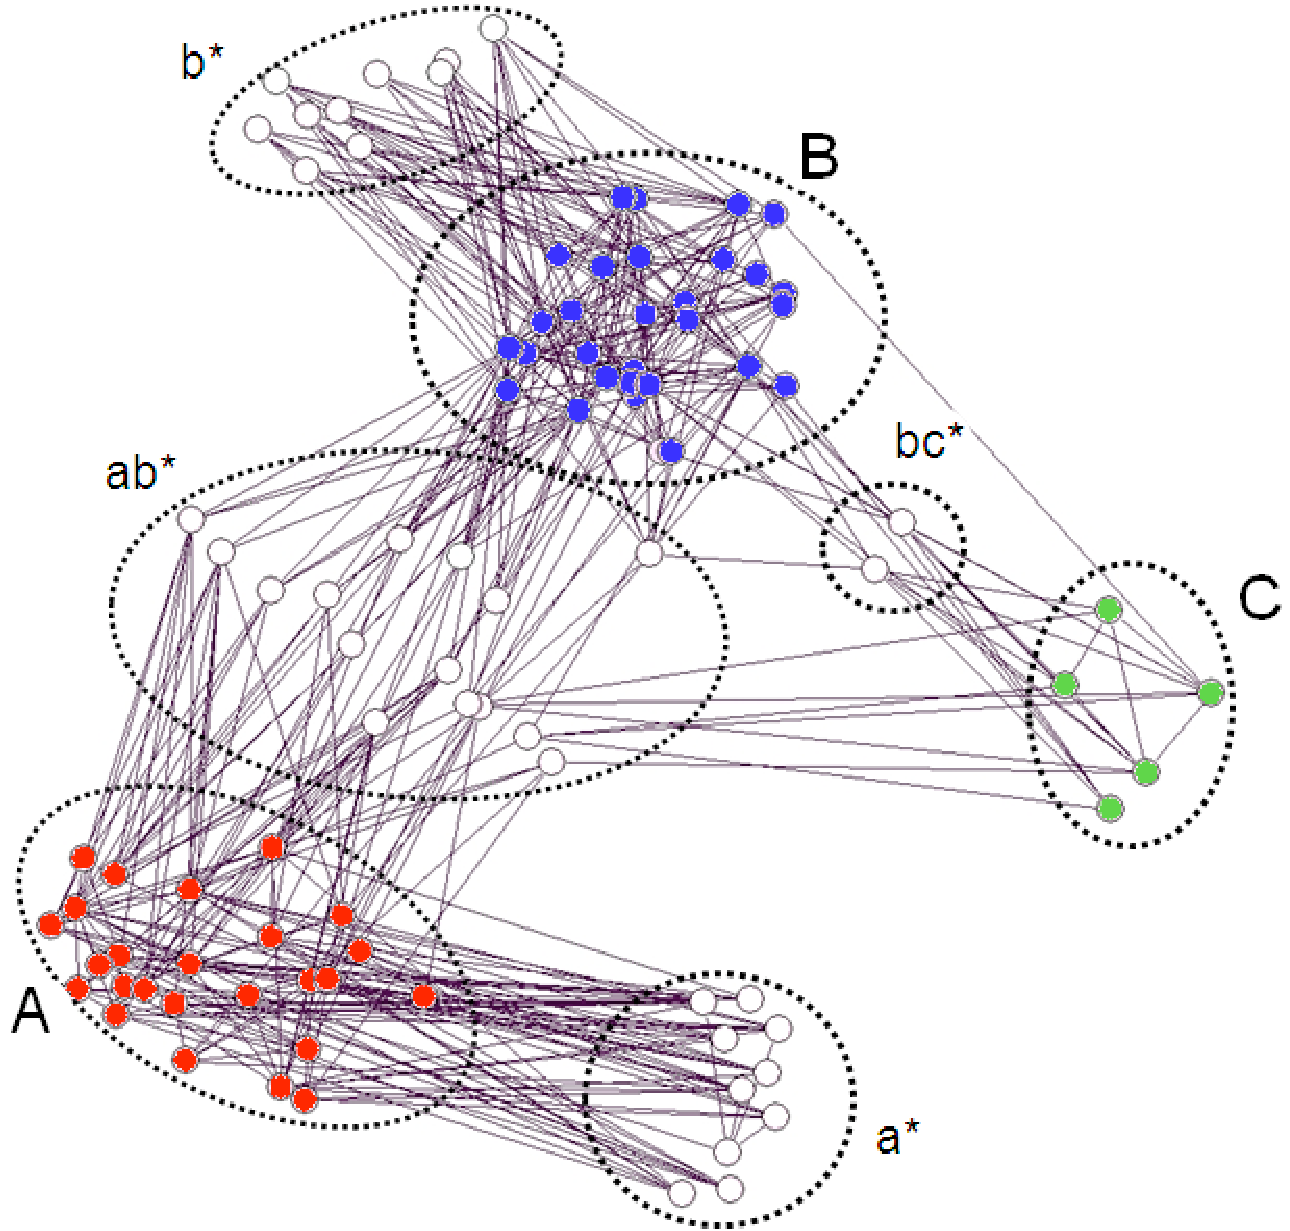
\includegraphics[width=0.8\columnwidth]{images/2002core_labelled}
\caption{Link reduction, showing Gangs A and B and emergence of
  Gang C (for 2002). This also illustrates the large amount of non-gang
  members who are associated with individual gangs (\emph{a*}, \emph{b*}) or who are intermediaries (\emph{ab*}, \emph{bc*}).}
\label{fig:2002core_labelled}
\end{figure}


\section{Network characterisation}\label{sec:networkcharacteristics}
A series of experiments were carried out to determine how the gang
networks compare with well-known networks, for example scale-free and
small-world networks.

\subsection{Small-world networks}\label{sec:smallworld}
Table~\ref{tab:networkmeasuresyears} presents the clustering
coefficient~\cite{WattsStrogatz1998} (CC) for each individual year,
alongside the node and edge counts and various other measures to
describe the network. For any simple connected graph \emph{G} with at
least two vertices, the clustering coefficient (1-neighbourhood)
\cite{WattsStrogatz1998} measures the extent to which vertices linked
to any given vertex \emph{v} are also linked to each other. Or in
other words, are the friends of my friends also my friends? This is
1-neighbourhood clustering. The clustering coefficient 2-neighbourhood
is a less stringent condition, and states: of the friends of my
friends, are they linked to me by other friends?

The links presented in Table~\ref{tab:networkmeasuresyears} are
cumulative; that is, the links and nodes for 2002 include not only the
new links and nodes for 2002, but also those for 2001 and 2000.

\begin{table}[htb]
\resizebox{\columnwidth}{!}{
\begin{tabular}{|l|r|r|r|r|r|r|r|}
\hline
 Measure &  2000 &  2001 &  2002 &  2003 &  2004 &  2005 &  2006 \\ 
\hline
 Number of nodes (n) &  1095 &  1295 &  1487 &  1752 &  2090 &  2229 &  2408 \\ 
\hline
 1/n &  0.00091 &  0.00077 &  0.00067 &  0.00057 &  0.00048 &  0.00045 &  0.00042 \\ 
\hline
 4/n &  0.00365 &  0.00309 &  0.00269 &  0.00228 &  0.00191 &  0.00180 &  0.00166 \\
\hline
 log(n) &  6.999 &  7.166 &  7.305 &  7.469 &  7.645 &  7.709 &  7.787 \\ 
\hline
 log(log(n)) &  1.95 &  1.97 &  1.99 &  2.01 &  2.03 &  2.04 &  2.05 \\ 
\hline
 Number of links &  1565 &  1903 &  2295 &  2844 &  3540 &  3872 &  4265 \\ 
\hline
 Total possible links &  598965 &  837865 &  1104841 &  1533876 &  2183005 &  2483106 &  2898028 \\ 
\hline
 Diameter &  12 &  14 &  11 &  11 &  14 &  12 &  13 \\
\hline
 Average path length &  4.85 &  4.82 &  4.68 &  4.57 &  4.86 &  4.78 &  4.70 \\ 
\hline
 Density &  0.00261 &  0.00227 &  0.00208 &  0.00185 &  0.00162 &  0.00156 &  0.00147 \\ 
\hline
 Betweenness &  0.107 &  0.117 &  0.172 &  0.205 &  0.146 &  0.102 &  0.100 \\ 
\hline
 CC (cumulative) &  0.47 &  0.48 &  0.47 &  0.46 &  0.49 &  0.55 &  0.56 \\ 
\hline
 CC (per year) &  0.24 &  0.57 &  0.34 &  0.15 &  0.62 &  0.25 &  0.30 \\ 
\hline
\end{tabular}}
\caption{Network measures for 2000-2006. Clustering coefficients are always greater than 4/n. Average path lengths are always less than log(n).}
\label{tab:networkmeasuresyears}
\end{table}


Table~\ref{tab:networkmeasuresgang} shows the same network measures,
but this time the data has been sliced into the members of the Gangs
A, B, C and D.


\begin{table}[htb]
\resizebox{\columnwidth}{!}{
\begin{tabular}{|l|r|r|r|r|}
\hline
 Measure & \multicolumn{1}{c|}{A} & \multicolumn{1}{c|}{B} & \multicolumn{1}{c|}{C} & \multicolumn{1}{c|}{D} \\
\hline 
 Number of nodes (n) &  859 &  617 &  431 &  513 \\ 
\hline
 1/n &  0.00116 &  0.00162 &  0.00232 &  0.00195 \\ 
\hline
 4/n &  0.00466 &  0.00648 &  0.00928 &  0.00780 \\ 
\hline
 log(n) &  6.76 &  6.42 &  6.07 &  6.24 \\ 
\hline
 log(log(n)) &  1.91 &  1.86 &  1.80 &  1.83 \\ 
\hline
 Number of links &  844 &  1047 &  602 &  707 \\ 
\hline
 Total possible links &  368511 &  190036 &  92665 &  249571 \\ 
\hline
 Diameter &  7 &  5 &  6 &  7 \\ 
\hline
 Average path length &  3.61 &  3.38 &  3.37 &  4.11 \\ 
\hline
 Density &  0.00396 &  0.00550 &  0.00648 &  0.00537 \\ 
\hline
 Closeness &  0.302 &  0.298 &  0.393 &  0.305 \\ 
\hline
 Betweenness &  0.185 &  0.179 &  0.350 &  0.239 \\ 
\hline
 CC &  0.16 &  0.19 &  0.15 &  0.12 \\ 
\hline
\end{tabular}}
\caption{Network measures for Gangs A, B, C, D. CC is the  average clustering coefficient from~\cite{WattsStrogatz1998}, considering only 1-neighbourhood.}
\label{tab:networkmeasuresgang}
\end{table}

A small-world network has both local connectivity and global
reach~\cite{WattsStrogatz1998}, and is a simple connected graph
\emph{G} exhibiting two properties:

\begin{enumerate}
\item Small characteristic path length: the presence of short-cut
connections between some vertices results in a small characteristic
path length \emph{L(G)}.
\item Large clustering coefficient: each vertex of \emph{G} is linked
to a relatively well-connected set of neighbouring vertices, resulting
in a large value for the clustering coefficient \emph{C(G)}.
\end{enumerate}
 
To determine whether our network is a random one or is small-world, we
can test whether or not it has exponential \emph{k}-connectivity
distribution. We do not observe this in the data, however, we do see
large clustering coefficients, and the average path lengths are always
less than {\emph{log(n)}}. Based upon these two criteria we can still
conclude that our networks have small-world characteristics.


\subsection{Scale-free networks}\label{sec:scalefree}
This section also refers to the preceding tables, where we find a
mixture of evidence for and against the case for scale-free networks.

Plotting the clustering coefficient as a function of the number of
nodes $n$, should follow the power-law distribution for scale-free
networks (see later experiments), with the clustering coefficient
being roughly four times larger than random networks
\cite{AlbAlbNak04}. The value of the clustering coefficient for a
random networks will be \emph{1/n}. In this way we are able to compare
the values of \emph{4/n} against CC in
Tables~\ref{tab:networkmeasuresyears} and
\ref{tab:networkmeasuresgang}. As the cumulative links increase from
2000 to 2006, the value of CC generally increases (with the number of
nodes n) and is always significantly higher than the values of
\emph{4/n}. Each of the gang values for CC are also significantly
higher than would be expected in a random network.

The diameter of the network (longest path length) should be
approximately \emph{log(log(n))} for scale-free networks. In both
cases (for the gangs and the years) the real values are significantly
higher than would be expected for a scale-free network. The average
path length should be approximately \emph{log(n)} for scale-free
networks. For both the `years' and `gangs' data it was actually
smaller than \emph{log(n)}, indicating scale-free networks.

The statistics on degree centrality were low, indicating that there is
no group leader. As we know when Gangs C and D are formed (2001
and 2004 respectively), it is interesting to note that the
characteristic of the networks at this time are that the betweeness
centralisation reaches 0.2. It is necessary to compare the closeness and
betweenness averages for each gang against the value for the overall
network.


\subsection{Power law investigation}\label{sec:powerlaw}



Our initial power law investigations used a log-log plot and $R^2$
values, and these all produced $\alpha$ values within this typical
range (between 2 and 2.5). However being roughly straight on a log-log
plot is a necessary but not sufficient condition for power-law
behaviour~\cite{ClausetShaliziNewman2009}, and that there are problems
(bias and inaccuracy) with fitting to the power-law distribution using
graphical methods based on linear fit on the log-log scale.

We therefore proceeded to use maximum likelihood estimation (MLE),
which is a far more robust method for estimating the scaling exponent
\cite{GoldsteinMorrisYen2004,ClausetShaliziNewman2009}. We report the
maximum likelihood estimate of the scaling exponent ($\alpha$), the
estimate of the lower bound of the power-law ($xmin$).

By optimising the Kolmogorov-Smirnov goodness-of-fit statistic, we can
use a \emph{goodness of fit} to estimate where the empirically-best
scaling region begins~\cite{ClausetShaliziNewman2009}. Given an
observed data set and a hypothesised power-law distribution from which
the data are drawn, we can then test whether our hypothesis is a
plausible one using the goodness-of-fit test (the Kolmogorov-Smirnov
statistic), given the data, and generate a p-value that quantifies the
plausibility of the hypothesis.

Employing the Kolmogorov-Smirnov test we are able to choose among the
hypotheses that: 

\begin{itemize}
\item \emph{H0}: the data follow a specified distribution;
\item \emph{Ha}: the data do not follow the specified distribution. 
\end{itemize}

We did not use Vuong's test to check for alternative distributions
(non-power-law distributions) which could have produced the
data. Instead, because our sample sizes are small (i.e., $< 100$), we
explicitly used an experimental finite-size correction, as recommended
by~\cite{ClausetShaliziNewman2009}.

Figure~\ref{fig:clausetcumulative} shows our results for our network
between 2000-2006. In all cases the exponent $\alpha$ is less than
2. Only when the power-law exponent is in the range $2--3$ do the
hubs tend to connect to form a single cohesive hierarchy
\cite{AdamicLukoseHuberman2003}.  The goodness-of-fit (gof) and
p-values however are significant. Even though the p-values are above
0.1 (arbitrary threshold level), we err on the side of caution because
of the low $\alpha$ value and the small sample size. When $n$ is
small, meaning $n \leq 100$, we cannot rule out the power-law
hypothesis \cite{ClausetShaliziNewman2009}. It is possible, for small
values of $n$, that the empirical distribution will follow a power law
closely, and hence that the p-value will be large, even when the power
law is the wrong model for the data
\cite{ClausetShaliziNewman2009}. 
%However, what we can say is that certainly the tail is heavy.

\begin{figure}[!ht]
\centering
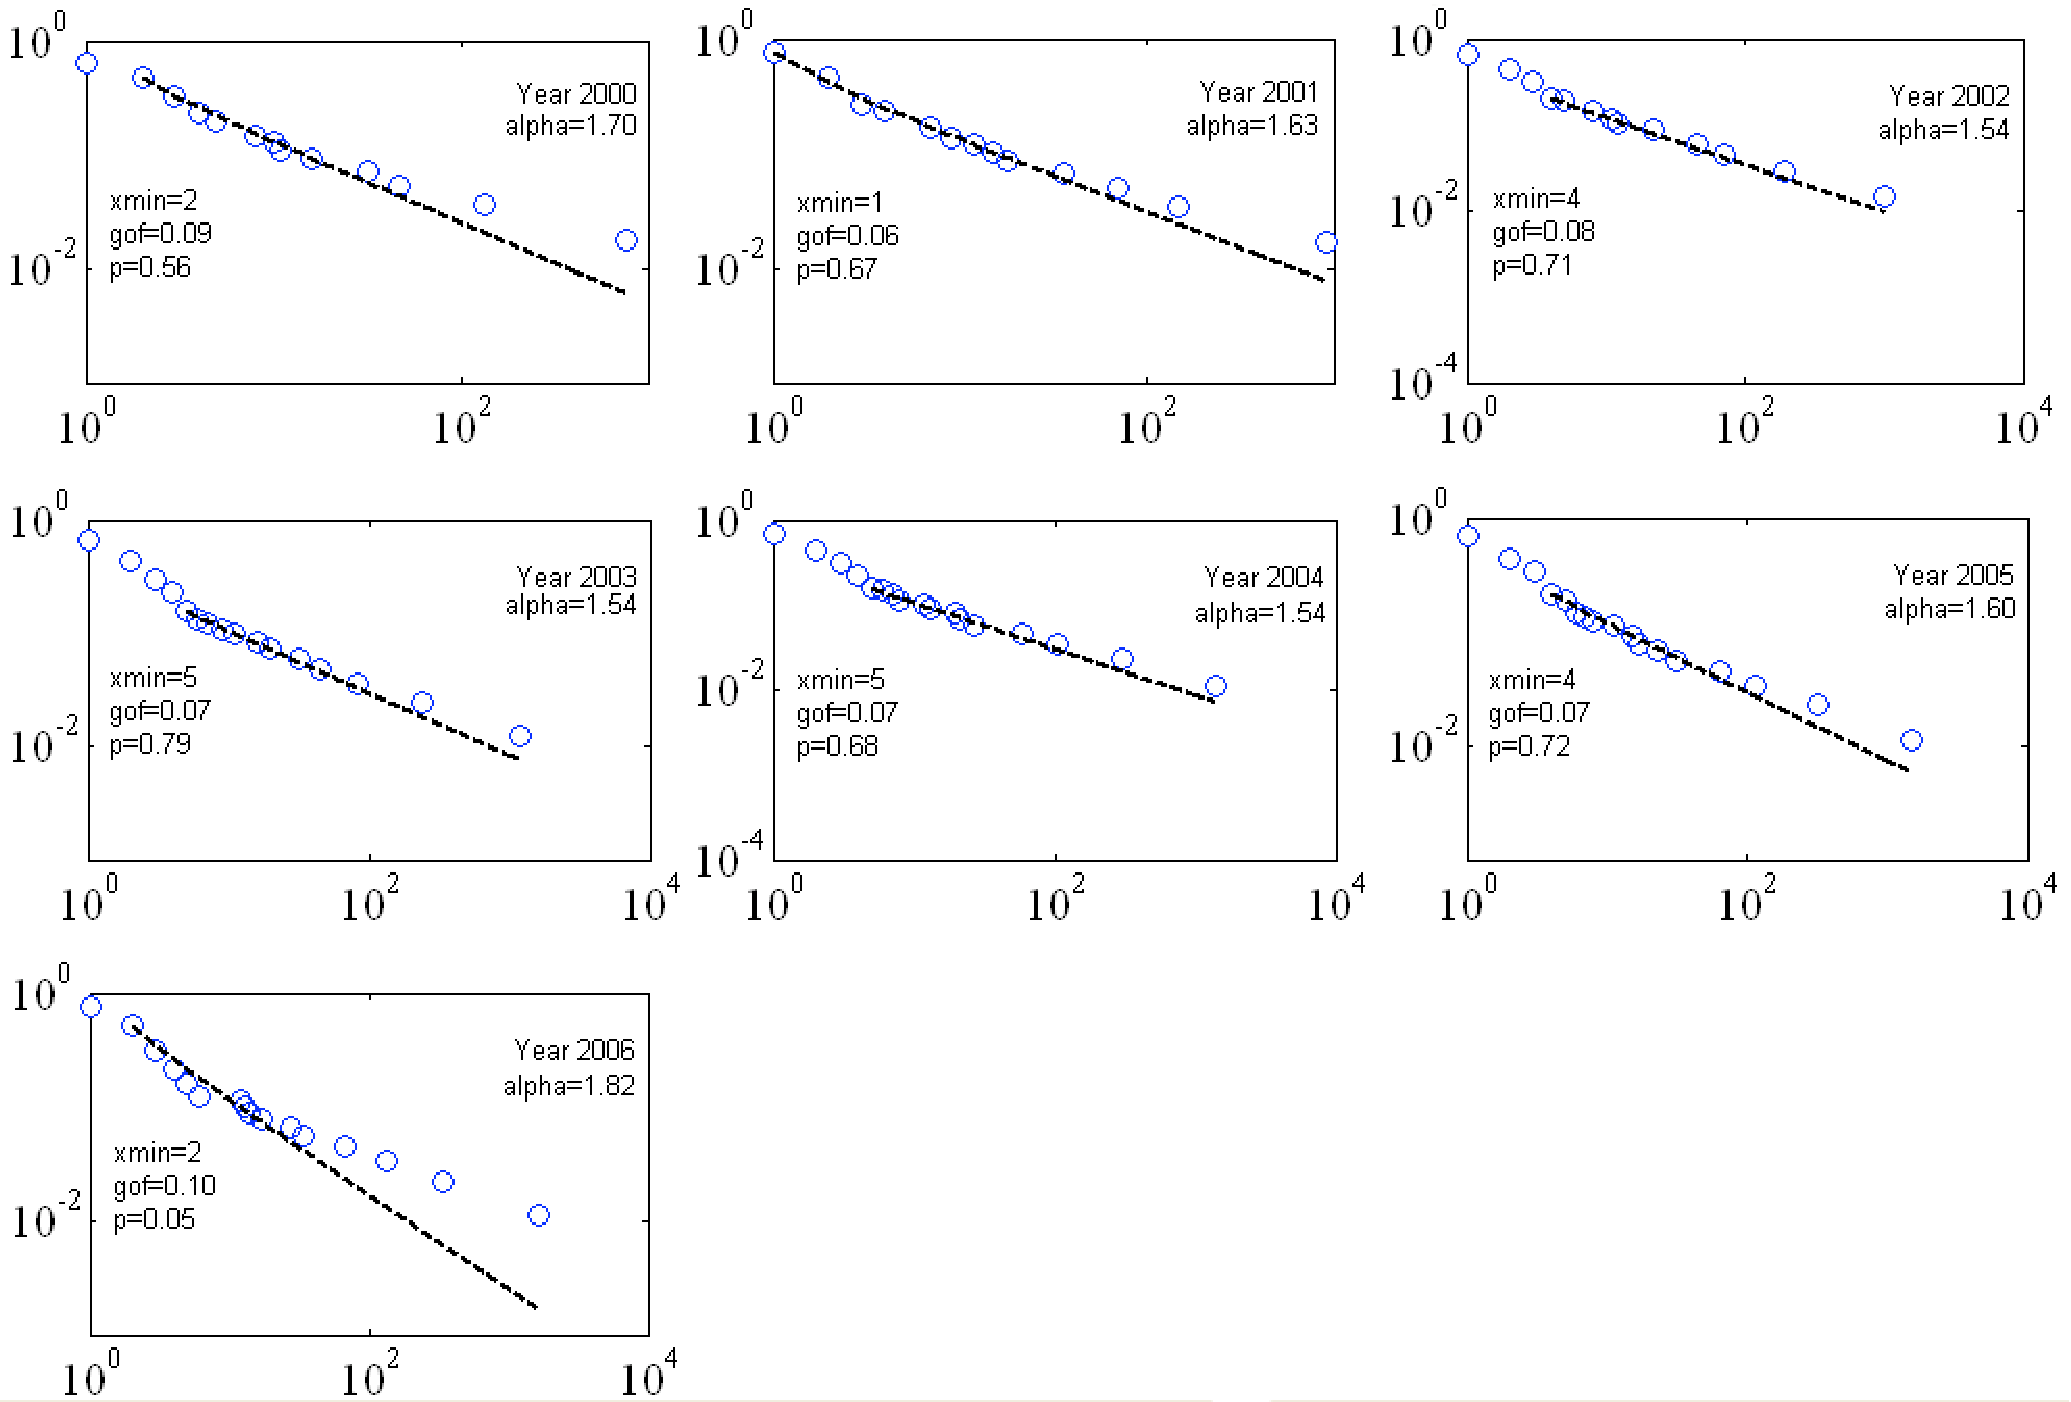
\includegraphics[width=\columnwidth]{images/clausetcumulative}
\caption{Power law investigations. A power law is fitted to each years data and various statistics calculated: the exponent alpha, xmin, goodness-of-fit (gof) and p-value.}
\label{fig:clausetcumulative}
\end{figure}

Table~\ref{tab:clausetgangyears} shows our results for the power law
exponent for the different gangs against years. The case is similar in
that there are significant gof and p-values, however in nearly all
cases the exponent is less than 2, and again we did not test for
alternate explanatory distributions, satisfied (operationally) that
the the tail was heavy in all cases, indicating the presence of very
well connected offenders.


\begin{table}[htb]
\resizebox{\columnwidth}{!}{
\centering
\begin{tabular}{|p{48pt}|l|l|l|l|l|l|l|l|l|}
\hline
\multicolumn{1}{|c|}{Gang} & 1999 & 2000 & 2001 & 2002 & 2003 & 2004 & 2005 & 2006 & 2007 \\
\hline
\multicolumn{1}{|c|}{A} & \textbf{2.65} &  1.47 & 1.00 & \textbf{1.91} & 1.07 & 0.10 & 0.94 & 0.77 & 0.74 \\
\hline
\multicolumn{1}{|c|}{B} & \textbf{2.95}& 1.44& \textbf{3.64}& \textbf{1.88}& 1.36& 0.09& 0.97& 0.63& 0.51 \\
\hline
\multicolumn{1}{|c|}{C} & 0.27& 0.24& 0.17& 0.32& 0.38& 0.02& 0.46& 0.36& 0.32 \\
\hline
\multicolumn{1}{|c|}{D} & 1.26& 0.76& 0.56& 0.69& 1.14& 0.03& 1.21& 0.81& 0.65 \\
\hline
\end{tabular}}
\caption{Power law exponents for gangs, against years (significant results are shown in bold).}
\label{tab:clausetgangyears}
\end{table}

Based on these experiments we are therefore unable to comment whether
the networks possessing scale-free characteristics, however we can
conclude that we have small-world networks, since consistently there
are larger clustering coefficients and shorter path lengths compared
to a random network with same number of gang members. This means two
things for our system:

\begin{itemize}
\item The smaller path length means that the criminal activity
(contagion) spreads more easily in this network than in a random
network.
\item Larger clustering coefficient means that contacts of contacts
are treated as contacts as well.
\end{itemize}


\subsection{Emergence of gangs}\label{sec:emergence}
We might see changes in the path length and clustering
coefficients from 2000 to 2005, indications of how the gangs have
become more closely knit or are splitting apart. By examining annual
links for 2001 and 2004, we might predict that the cumulative links
decrease and the annual links increase, just before/as a gang forms,
then both values increase afterwards as everyone becomes linked
together. This is not the case, and neither are we able to see any
meaningful behaviour in these data.

Figure~\ref{fig:gangscc1years} shows the clustering
coefficients for each gang and against years. In Table~\ref{fig:gangscc1years} the
CC value of each gang dips at 2004. What this may indicate is
clustering due to non-gang members (from
Figure~\ref{fig:2002core_labelled}, offenders who are connected to
gang members: \emph{a*}, \emph{b*}, \emph{bc*} and \emph{ab*}) and
less clustering that previous years between members of gangs
themselves. There is also a significant peak in clustering during 2001
for Gang B, whereas all other gangs suffer a decrease in clustering.



\begin{figure}[htb]
\centering
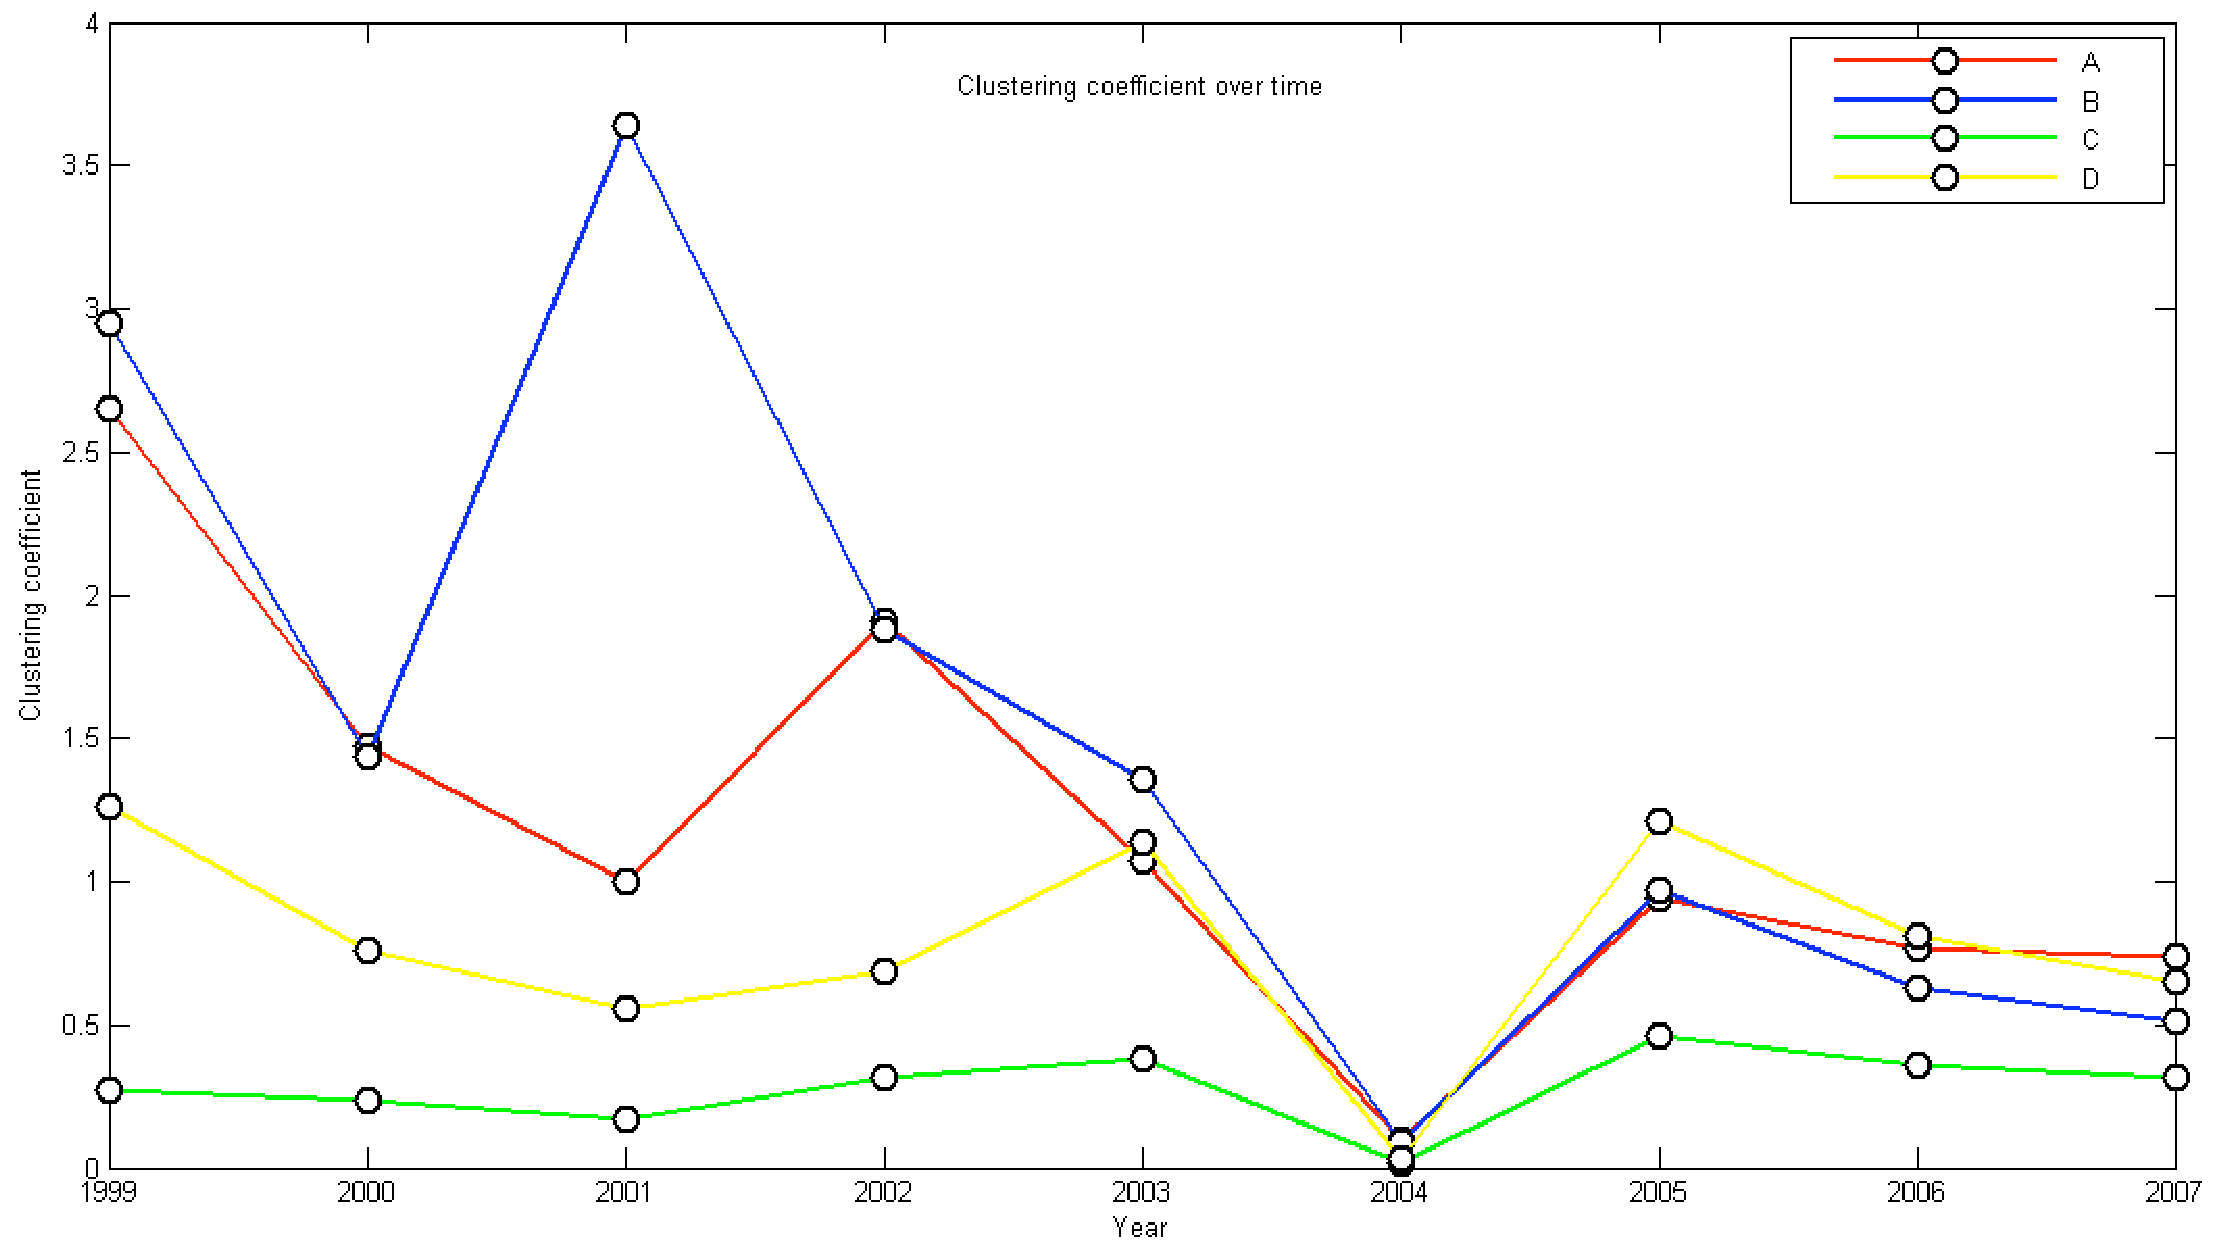
\includegraphics[width=\columnwidth]{images/gangscc1years}
\caption{Per year clustering coefficients for each gang. Gang C was formed in 2001, Gang D in 2004.} 
\label{fig:gangscc1years}
\end{figure}


\section{Discussion}\label{sec:discussion}
The model of two rival sets of gangs is potentially a
misrepresentation of the much more complex sets of smaller cliques and
fluid changes within the larger gang structures. However, the four
gangs discussed do exist, and are the main gangs; what is not possible
is a high degree of exactitude.

%\subsection{External and internal factors}

We require a much better analysis of link types, developed a model
where individuals learn about crime opportunities by interacting with
other peers; for instance whether weak ties play an important role in
explaining criminal activities~\cite{PatacchiniZenou2008}, especially
gang homicide~\cite{papachristos:2009}. The theoretical predictions of
the model are confirmed by the empirical analysis since they find that
weak ties, as measured by friends of friends, have a positive impact
on criminal activities.

Furthermore, for 2001 and 2004, it would be interesting to examine the
kinds of links within each gang which split apart.


\section{Conclusions}\label{sec:conclusion}
The work presented in this paper contains our initial findings about
the offender/gang networks in Manchester in the UK, using network
analysis. The uses of this technology in an operational context are
significant. Even using the networks merely as visual representations
of otherwise cognitively unmanageable data contained in spreadsheets
and databases is operationally very useful, for knowledge sharing and
training, and identifying key offenders. When further pre-processing
is carried out, and the quality of the data collection process is
improved, there will be sigificant future work available with this
dataset.

The police crime recording database is routinely gathered and
available for analysis. The additional databases of histories and
associates of gang offenders are routinely gathered by the UK's
National Crime
Agency~\footnote{\url{http://www.nationalcrimeagency.gov.uk/}}, who
investigate gang and gun-related crimes. These data sources are
potential rich sources of information for computer science
technologies to deliver crime prevention and detection decision
support systems.



% \section*{Acknowledgments}
% We acknowledge the UK's Engineering \& Physical Sciences Research
% Council (EPSRC) Sandpit on Gun Crime (September 2005, Warwickshire,
% UK), funded by the IDEAS Factory; and the assistance of Xcalibre, the Greater
% Manchester Police's specialist gang crime task force.

% trigger a \newpage just before the given reference
% number - used to balance the columns on the last page
% adjust value as needed - may need to be readjusted if
% the document is modified later
%\IEEEtriggeratref{37}
% The "triggered" command can be changed if desired:
%\IEEEtriggercmd{\enlargethispage{-5in}}

% BibTeX users
\bibliographystyle{IEEEtran}      % basic style, author-year citations
\bibliography{asonam2014}   % name your BibTeX data base

\end{document}
% end of file template.tex

